In this lab we solve combinational optimization problems using integer and dynamic programming.
\subsection{N Queens}
The N queens puzzle is the problem of placing N chess queens on an $N\times N (N\ge 4)$ chessboard so that no two queens threaten each other; thus, a solution requires that no two queens share the same row, column, or diagonal.

The constraints for the rows and columns are trivial to implement. The constraint for the diagonals can be implemented by checking if the difference between the row and column of two queens is the same (main diagonal) or the sum is the same (secondary diagonal).
Below an example of the N queens problem for $N=10$ is shown.
\begin{figure}[H]
    \centering
    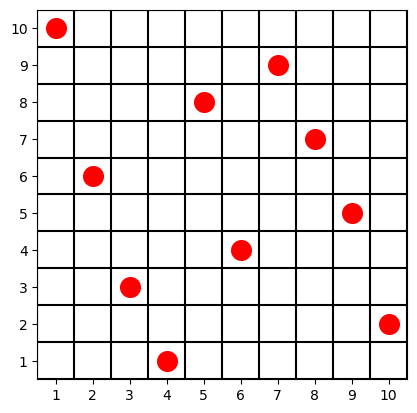
\includegraphics[width=0.7\textwidth]{lab11/imgs/nqueens.png}
    \caption{N queens problem for $N=10$}
    \label{fig:nqueens}
\end{figure}

\subsection{TSP}
The goal of the TSP is to find the shortest Hamiltonian cycle (a cycle that visits each node only once) on a graph of $N$ nodes. The formulation for integer programming is as follows:
\begin{align*}
    \text{minimize}   & \sum_{i=1}^{N}\sum_{j=1}^{N}d_{ij}x_{ij}                &                            \\
    \text{subject to} & \sum_{j=1}^{N}x_{ij} = 1, \quad i=1,\ldots,N            & \text{one predecessor}     \\
                      & \sum_{i=1}^{N}x_{ij} = 1, \quad j=1,\ldots,N            & \text{one successor}       \\
                      & u_1 = 1                                                 & \text{starting node}       \\
                      & u_i - u_j +1 \leq (N-1)(1-x_{ij}), \quad i,j=2,\ldots,N & \text{subtour elimination}
\end{align*}
where $d_{ij}$ is the distance between node $i$ and $j$, $x_{ij}$ is a binary variable that is 1 if the path goes from node $i$ to node $j$, and $u_i$ is a auxiliary variable that represents the position of node $i$ in the cycle.

Below an example of the TSP problem for $N=10$ is shown.
\begin{figure}[H]
    \centering
    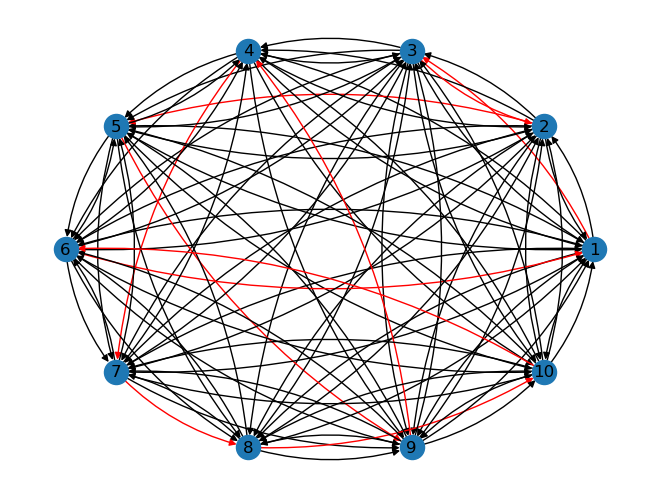
\includegraphics[width=0.7\textwidth]{lab11/imgs/tsp.png}
    \caption{TSP problem for $N=10$}
    \label{fig:tsp}
\end{figure}

\subsection{Knapsack}
The goal of the knapsack problem is to maximize the value of the items in the knapsack without exceeding the volume capacity. We'll solve it using dynamic programming and tabulation.

\begin{lstlisting}
def knapsack(W, wt, val, n):
    DP = [[0 for _ in range(W+1)] for _ in range(n+1)]
    for i in range(n+1):
        for w in range(W+1):
            if i == 0 or w == 0: # base case
                DP[i][w] = 0
            elif wt[i-1] <= w:
                # decide if we take the item or not
                DP[i][w] = max(val[i-1] + DP[i-1][w-wt[i-1]], DP[i-1][w])
            else:
                # we can't take the item
                DP[i][w] = DP[i-1][w]
    return DP[n][W] # return the maximum value
\end{lstlisting}

\paragraph*{Example for the knapsack problem}
Given the following items:
\begin{table}[H]
    \centering
    \begin{tabular}{c|c|c|c|}
        Item & Volume     & Value      \\ \hline
        01   & apple      & 2     & 1  \\
        02   & pear       & 2     & 2  \\
        03   & banana     & 2     & 2  \\
        04   & watermelon & 5     & 10 \\
        05   & orange     & 2     & 3  \\
        06   & avocado    & 2     & 3  \\
        07   & bluberry   & 1     & 3  \\
        08   & coconut    & 3     & 4  \\
        09   & cherry     & 1     & 2  \\
        10   & apricot    & 1     & 1  \\
        \hline
    \end{tabular}
\end{table}

We compare the results for different knapsack capacities and we can see that the algorithm works as expected, achieving the maximum capacity for all cases except for $C=20$.
\begin{table}[H]
    \centering
    \begin{tabular}{c|c|c|c|c|c|c|c|c|c|c|c|}
        Capacity & Achieved Capacity & Value & Items in the knapsack      \\ \hline
        5        & 5                 & 9     & 05 06 07                   \\
        10       & 10                & 16    & 05 06 07 08 09 10          \\
        15       & 15                & 20    & 01 02 03 05 06 07 08 09    \\
        20       & 16                & 21    & 01 02 03 05 06 07 08 09 10 \\
        25       & 25                & 25    & 01 02 03 04 05 06 07 08 09 \\
    \end{tabular}
\end{table}